\documentclass[10pt,letterpaper]{scrartcl}
\usepackage{amsfonts,amsmath,amssymb}
\usepackage{dsfont,fontawesome}
\usepackage{braket,mathtools,siunitx}
\usepackage[hidelinks]{hyperref}
\usepackage{textcomp,url}
\usepackage{xcolor,graphicx,tikz,pgfplots}
\definecolor{shadecolor}{rgb}{0.9,0.9,0.9}
\usetikzlibrary{arrows}
\pgfplotsset{compat=1.12}
\usepackage{listings,enumerate}
\usepackage{booktabs,tabularx,longtable,multicol}
\usepackage[inner=2cm,outer=2cm,top=2cm,bottom=2.3cm]{geometry}

\pagestyle{empty}
\setlength{\parindent}{0pt}
\setlength{\parskip}{6pt}

\newcommand{\dx}{\;\mathrm{d}x}
\newcommand{\ds}{\;\mathrm{d}s}
\renewcommand{\div}{\operatorname{div}}

\begin{document}

\begin{minipage}{.2\textwidth}
\includegraphics[width=42pt]{ubc-logo.png}
\end{minipage}
\hfill
\begin{minipage}{.75\textwidth}
\setlength{\parskip}{6pt}
\begin{flushright}
{
\sffamily
\textbf{MATH521: Numerical Analysis of Partial Differential Equations}\\
Winter 2018/19, Term 2

Due Date: Thursday, 14 February 2019\\
Timm Treskatis
}
\end{flushright}
\end{minipage}

\section*{Homework Assignment 6}

Please submit the following files as indicated below: \hfill \faFileCodeO \: source code \hfill \faFilePdfO \: PDF file \hfill \faFilePictureO \: image file \hfill \faFileMovieO \: video file

\paragraph*{Question 1 $\vert$ 2 marks $\vert$ \faFilePdfO}

Given three points $a,b,c \in \mathds{R}^2$ that are not collinear (not all on one line) and that are sorted in anticlockwise order, we define
\begin{align*}
T &= \Delta(a,b,c) \qquad \text{(the triangle with these vertices)}\\
P &= P_2(T)\\
L &= \Set{ p\mapsto p(a), \quad
 p\mapsto p(b),\quad
 p\mapsto p(c),\quad
 p\mapsto \frac{\partial p}{\partial n}\left(\frac{a+b}{2}\right),\quad
 p\mapsto \frac{\partial p}{\partial n}\left(\frac{b+c}{2}\right),\quad
 p\mapsto \frac{\partial p}{\partial n}\left(\frac{c+a}{2}\right)} \subset P^*
\end{align*}

\begin{center}
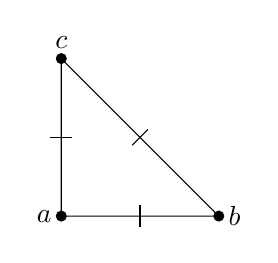
\begin{tikzpicture}
\draw (0,0) node[anchor=east]{$a$}
  -- (2,0) node[anchor=west]{$b$}
  -- (0,2) node[anchor=south]{$c$}
  -- cycle;
\fill (0,0) circle[radius=2pt];
\fill (2,0) circle[radius=2pt];
\fill (0,2) circle[radius=2pt];
\draw (1,-0.14) -- (1,0.14);
\draw (-0.14,1) -- (0.14,1);
\draw (1-0.1,1-0.1) -- (1+0.1,1+0.1);
\end{tikzpicture}
\end{center}

\begin{enumerate}[(a)]
\item Show that given any data for
\begin{equation*}
p(a), \quad
p(b),\quad
p(c),\quad
\frac{\partial p}{\partial n}\left(\frac{a+b}{2}\right),\quad
\frac{\partial p}{\partial n}\left(\frac{b+c}{2}\right)\quad \text{and} \quad
\frac{\partial p}{\partial n}\left(\frac{c+a}{2}\right)
\end{equation*}
there exists a unique interpolant $p \in P$.

\emph{1\textsuperscript{st} Hint:} Where does a parabola with $p(a)=0$ and $p(b) = 0$ have its vertex?

\emph{2\textsuperscript{nd} Hint:} There is a video on checking unisolvence in the Media Gallery.
\newpage

\item Now let $\Omega^h$ be a domain with a regular triangulation $\mathcal{T}^h$ such that
\begin{equation*}
\bar{\Omega}^h = \bigcup_{T\in \mathcal{T}^h} T.
\end{equation*}
Show that the space
\begin{equation*}
V^h = \Set{v^h: \bar{\Omega}^h\to \mathds{R} | \left. v^h\right\rvert_T \in P_2(T), v^h \text{ is continuous in all vertices}, \frac{\partial v^h}{\partial n} \text{ is continuous in all edge midpoints} }
\end{equation*}
is not $H^1$-conforming by giving me a specific example of a function $v^h \in V^h$ that has a jump across a triangle edge.
\end{enumerate}
\newpage

\paragraph*{Question 2 $\vert$ 3 marks $\vert$ \faFileCodeO \: \faFilePictureO \: \faFilePdfO}

We will now complete our finite-element solver for the linear elasticity problem
\begin{equation}\label{eq:le}
\begin{aligned}
-c\Delta u + a u &= f &&\text{in } \Omega\\
u &= g && \text{on } \partial\Omega.
\end{aligned}
\end{equation}

\begin{enumerate}[(a)]
\item Remove lines 1-10 from \texttt{discretiseLinearElasticity.m} and uncomment the sections of code that are currently commented out. Complete the missing commands, including the subfunction \texttt{assembleStiffness}. Also inspect the \texttt{assembleLoad} subfunction. Remember that you may use the code from last week's model answers if you are unsure whether your own code works correctly.
\item Write a script \texttt{hw6.m} which
\begin{itemize}
\item solves the linear elasticity problem on $\Omega^h$, which you may choose from \texttt{kiwi.mat}, \texttt{maple.mat}, \texttt{pi.mat}, \texttt{ubc.mat}. You may also select your own data for $f(x_1,x_2)$, $g(x_1,x_2)$, $a$ and $c$.

\emph{Hint:} You have to set \texttt{GammaD = @(x1,x2) true(size(x1))}. For debugging, you might want to use \texttt{video.mat} and check the sparsity patterns of the various matrices.
\item calculates the $L^2$, $H^1$ and energy norms
\begin{align*}
\lVert u^h \rVert_{L^2} &= \sqrt{\int\limits_{\Omega^h} \lvert u^h \rvert^2 \dx}\\
\lVert u^h \rVert_{H^1} &= \sqrt{\lVert u^h \rVert_{L^2}^2 + \lVert \nabla u^h \rVert_{L^2}^2} = \sqrt{\int\limits_{\Omega^h} \lvert u^h \rvert^2 \dx + \int\limits_{\Omega^h} \lvert \nabla u^h \rvert^2 \dx}\\
\lVert u^h \rVert_{B} &= \sqrt{B(u^h,u^h)} = \sqrt{c\int\limits_{\Omega^h} \lvert \nabla u^h \rvert^2 \dx + a \int\limits_{\Omega^h} \lvert u^h \rvert^2 \dx}
\end{align*}
of the solution, where $B$ is the bilinear form corresponding to the elliptic operator
\item creates undistorted plots of the mesh, the force $f$ and the solution $u^h$ (including the boundary points). Post your plots of $f$ and $u^h$ in the discussion forum!
\end{itemize}
\item What problem do you solve numerically when you set \texttt{GammaD = @(x1,x2) false(size(x1))}? Analyse the code to infer its weak formulation:
\end{enumerate}

\vfill

\paragraph*{So that you don't get bored during the break\dots}

Install \textsf{FEniCS} and \textsf{ParaView} on your computer and bring it with you to our first class after the break on Tuesday 26 February. Please make sure everything is set up and running before that date. Both \textsf{FEniCS} and \textsf{ParaView} are free and open source software.

\begin{description}
\item[FEniCS on Ubuntu Linux or Windows 10] Follow the instructions here: \url{https://fenicsproject.org/download/}.
\item[FEniCS on other Linux distributions, older versions of Windows or macOS] It will be easiest to use \textsf{FEniCS} on \textsf{Docker}. Follow the installation instructions here: \url{https://fenics-containers.readthedocs.io/en/latest/quickstart.html}.
\item[ParaView on Linux] \textsf{ParaView} should already be included in the official repositories of your distribution.
\item[ParaView on other operating systems] Download it here: \url{https://www.paraview.org/download/}.
\end{description}
If you need help with troubleshooting, there is a discussion thread on \textsf{Canvas}.

\paragraph*{Your Learning Progress $\vert$ 0 marks, but -1 mark if unanswered $\vert$ \faFilePdfO}
What is the one most important thing that you have learnt from this assignment?

% These lines are just here for the folks who submit handwritten answers. As you seem to type up your answers, just delete the lines :)
\vspace*{3mm}
\hrulefill

\vspace*{3mm}
\hrulefill

\vspace*{3mm}
\hrulefill

What is the most substantial new insight that you have gained from this course this week? Any \emph{aha moment}?

\vspace*{3mm}
\hrulefill

\vspace*{3mm}
\hrulefill

\vspace*{3mm}
\hrulefill

\end{document}